\chapter{INTRODUCTION}\
\pagenumbering{arabic}
\section{Motivation and Scope}
\hspace*{0.3in}The rapid evolution of both Quantum Computing (QC) and Artificial Intelligence (AI) has marked the beginning of a new computational era. While QC promises unprecedented power by leveraging the principles of quantum mechanics, AI continues to reshape industries through intelligent automation, data-driven insights, and problem-solving capabilities. The motivation for this study lies in the emerging convergence of these two domains—Quantum Artificial Intelligence (QAI)—which holds the potential to redefine not only computational efficiency but also how humanity approaches some of its most pressing challenges, such as climate change modeling, drug discovery, cybersecurity, and financial optimization.

The scope of this report is to examine how AI can accelerate the practical deployment of quantum systems, while quantum technologies, in turn, enhance AI performance on tasks that are computationally intractable for classical systems. This synergy represents an exciting frontier that demands exploration from researchers, practitioners, and policymakers alike.\\
\section{Definitions}
\begin{itemize}
	\item \textbf{Quantum Computing (QC)}: A computational paradigm that uses qubits instead of classical bits, enabling operations based on superposition, entanglement, and quantum interference. Unlike classical systems, QC can explore vast solution spaces in parallel, making it particularly powerful for problems such as optimization, cryptography, and molecular simulation.
	\item \textbf{Artificial Intelligence (AI):} A broad field of computer science concerned with building systems that exhibit human-like intelligence. Through techniques such as machine learning (ML), deep learning, and reinforcement learning (RL), AI enables machines to learn from data, adapt to new inputs, and perform complex decision-making tasks.
	\item \textbf{Quantum Artificial Intelligence (QAI):} The interdisciplinary domain where AI and QC intersect. QAI involves (i) applying AI methods to improve quantum technologies (e.g., calibration, error correction, control systems), and (ii) using quantum computers to accelerate or enhance AI algorithms (e.g., quantum machine learning, quantum optimization, quantum-enhanced natural language processing).
\end{itemize}
\begin{figure}
	\centering
	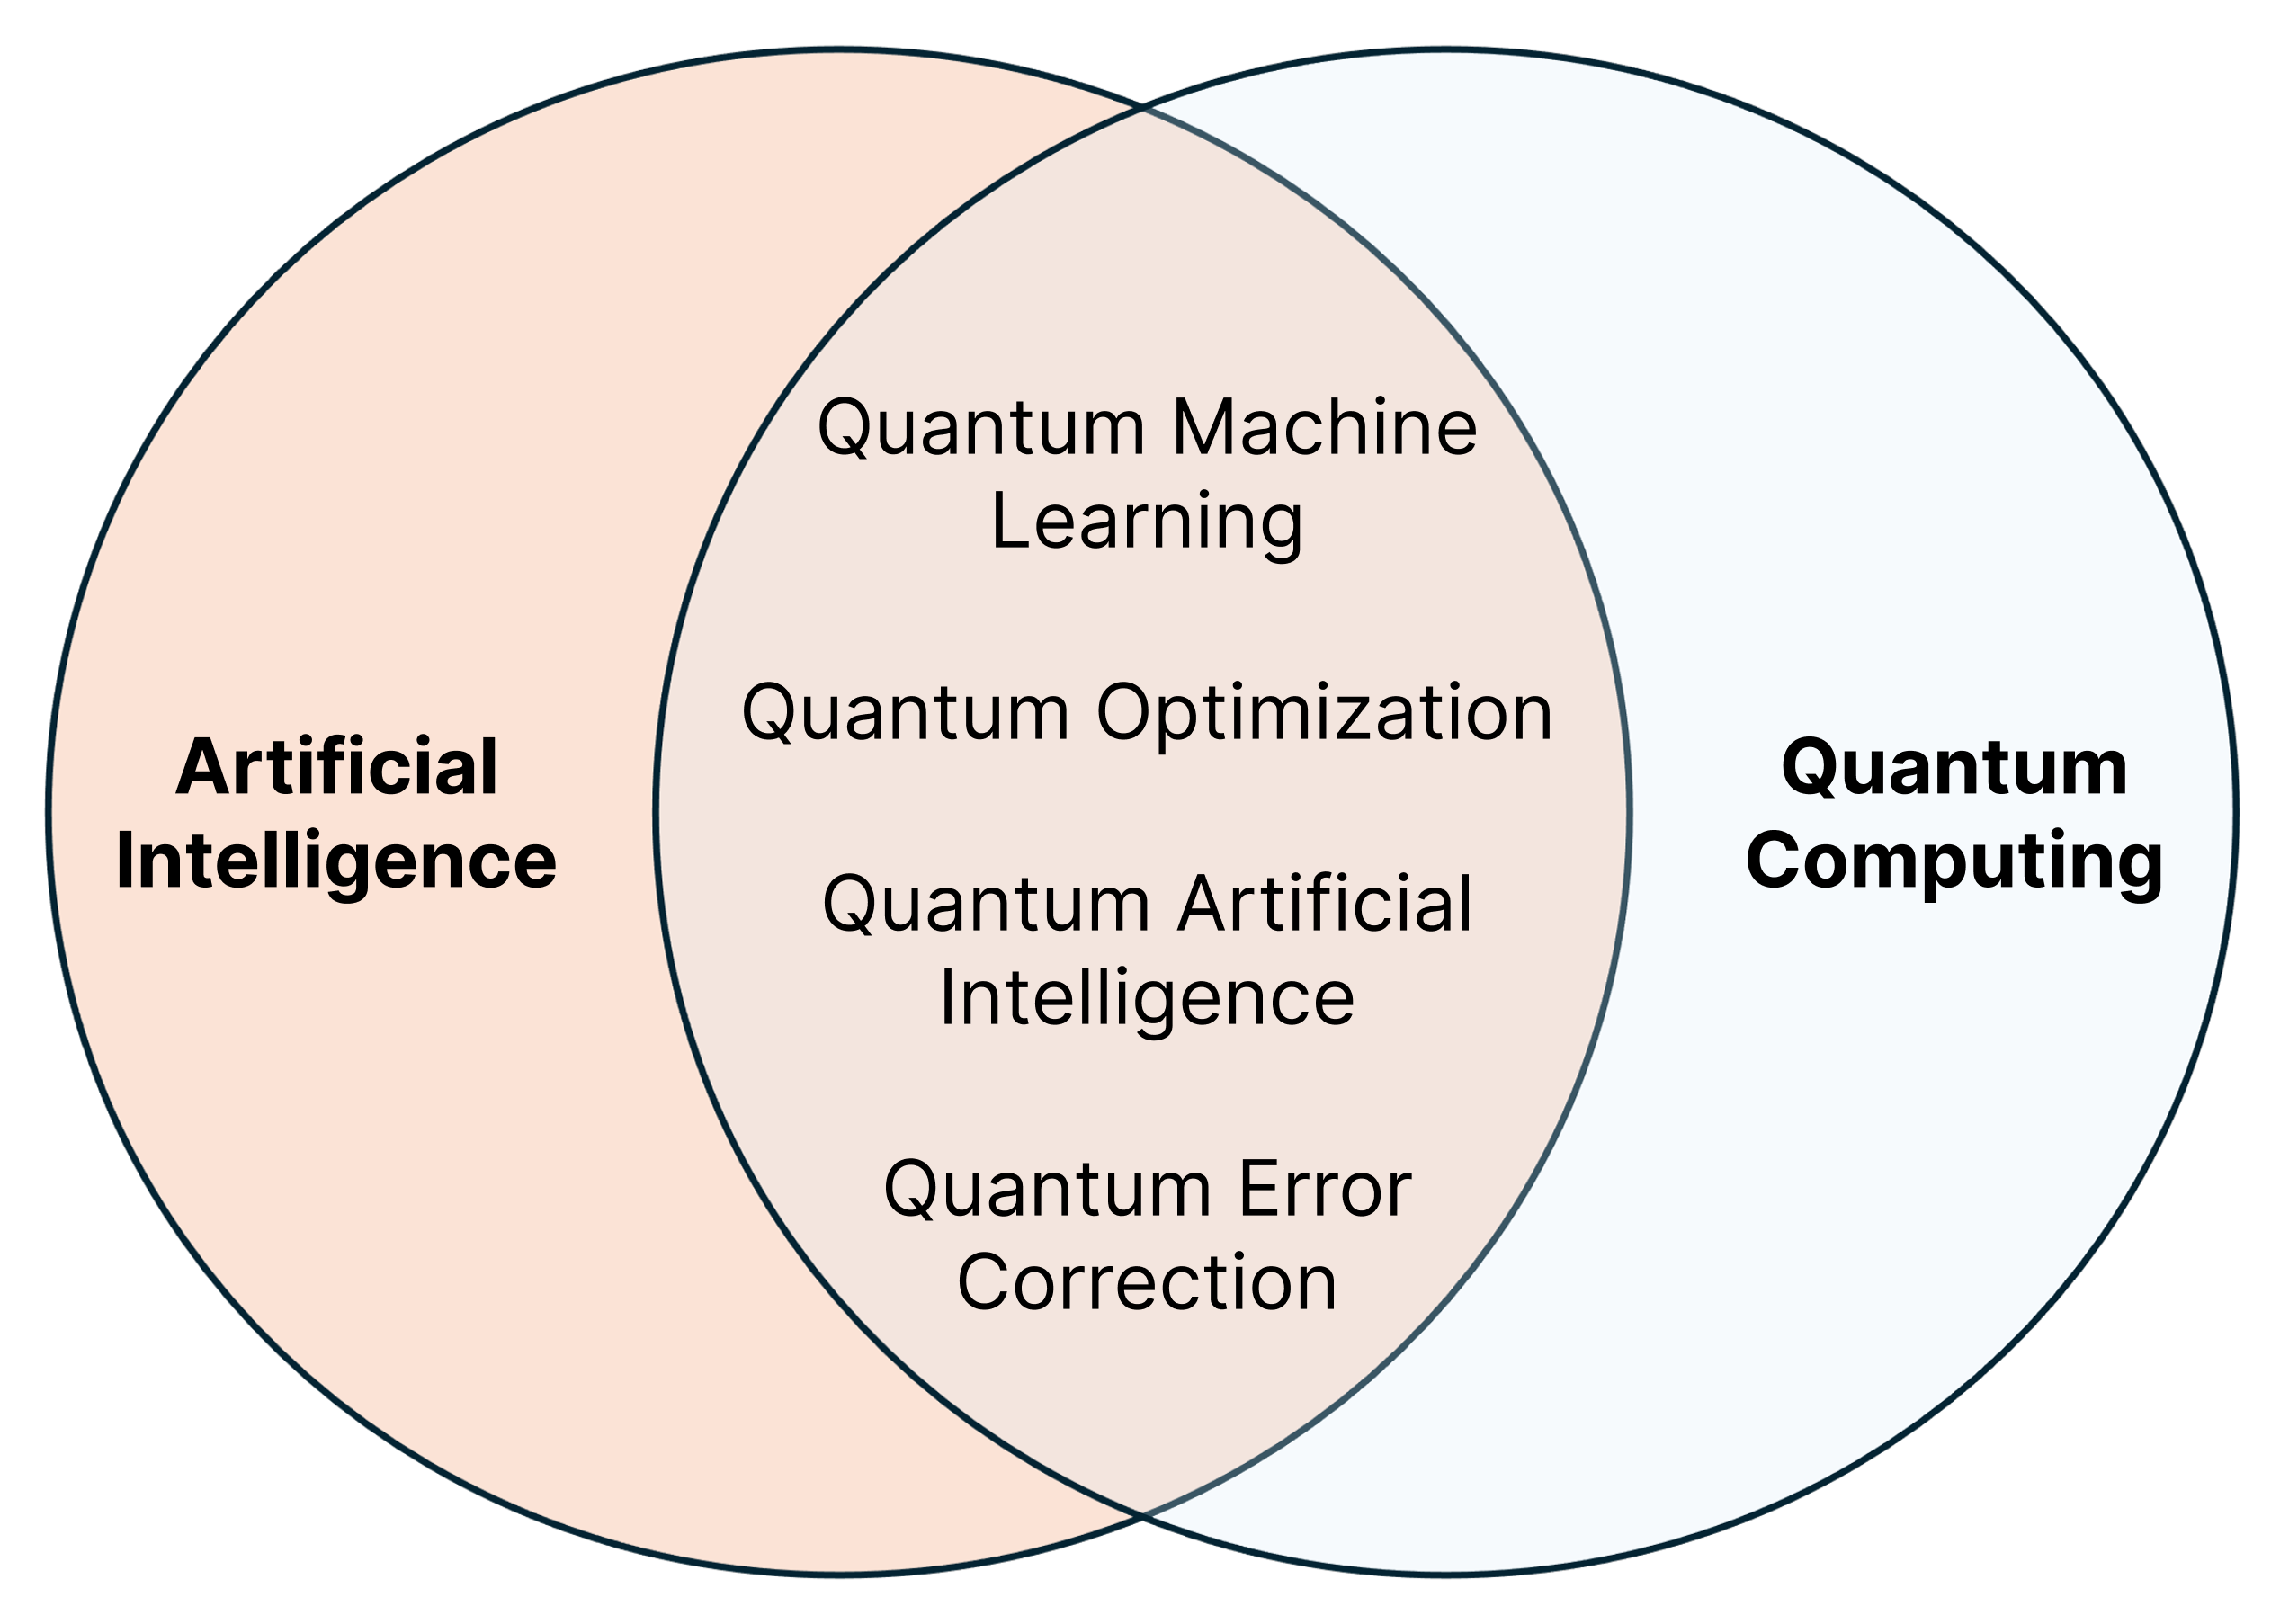
\includegraphics[width=1\linewidth]{QAI.png}
	\caption{Synergy of Artificial Intelligence and Quantum Computing}
	\label{fig:enter-label}
\end{figure}
\section{Objectives and Structure of the Report}
\hspace*{0.3in}This report reviews how Quantum Computing (QC) and Artificial Intelligence (AI) are converging into Quantum AI (QAI). It focuses on three goals:
\begin{enumerate}
	\item Outline key foundations and recent research trends.
	\item Highlight applications in areas like system design, error correction, NLP, healthcare, and finance.
	\item Discuss challenges, industry impacts, and future directions toward 2029.
\end{enumerate}

